\paragraph{QuizziPedia::Back-End::App::Models::Session}
\label{QuizziPedia::Back-End::App::Models::Session}
\begin{figure}[ht]
	\centering
	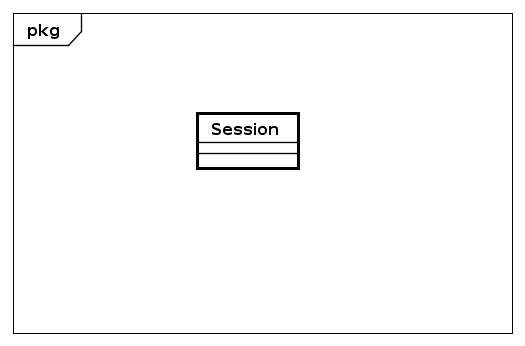
\includegraphics[scale=0.45]{UML/Classi/Back-End/QuizziPedia_Back-End_App_Models_sessionModel.png}
	\caption{QuizziPedia::Back-End::App::Models::Session}
\end{figure}
\FloatBarrier
	\begin{itemize}
		\item \textbf{Descrizione}: classe che gestisce la sessione utente dell'applicazione. Non sono stati modellati attributi e metodi di questa classe in quanto viene inizializzata da \textit{Express\ped{G}} ed utilizzata da \textit{Passport\ped{G}} attraverso funzionalità interne ai due \textit{middleware\ped{G}};
		\item \textbf{Utilizzo}: viene utilizzata da \textit{Passport\ped{G}} per memorizzare i dati della sessione che viene creata quando un utente effettua il login;
		\item \textbf{Relazioni con altre classi}:
			\begin{itemize}
				\item
				IN \texttt{AuthenticationController} \\
				Classe che si occupa della registrazione e dell'autenticazione dell'utente nel sistema. È un componente ConcreteHandler del design pattern \textit{Chain of responsibility\ped{G}}. Risulta essere il componente che eventualmente esegue la richiesta del client attraverso \textit{Passport\ped{G}};			
				\item
				IN \texttt{SessionController} \\
				Classe \textit{middleware\ped{G}} che, utilizzando \textit{Passport\ped{G}}, si occupa di controllare la consistenza dell'oggetto session durante la sessione associata all'utente autenticato. È un componente ConcreteHandler del design pattern \textit{Chain of responsibility\ped{G}}.
			\end{itemize}
	\end{itemize}